\documentclass[11pt]{article}
% \pagestyle{empty}

\usepackage{times}
\usepackage{mathptm}

\setlength{\oddsidemargin}{-0.3 in}
\setlength{\evensidemargin}{-0.3 in}
\setlength{\topmargin}{-1.05 in}
\setlength{\textwidth}{7.0 in}
\setlength{\textheight}{9.0 in}
\setlength{\headsep}{0.5 in}
\setlength{\parindent}{0.3 in}
\setlength{\parskip}{0.05 in}
\usepackage{epsf}
\usepackage{graphicx}

\def\O{\mathop{\smash{O}}\nolimits}
\def\o{\mathop{\smash{o}}\nolimits}
\newcommand{\e}{{\rm e}}
\newcommand{\R}{{\bf R}}
\newcommand{\Z}{{\bf Z}}


\begin{document}
	
	\section*{CS 124 Homework 7: Spring 2021}
 		
	\textbf{Your name:} 
		
	\textbf{Collaborators:} 

	\textbf{No. of late days used on previous psets: }\\
	\textbf{No. of late days used after including this pset: }

Homework is due Friday 2021-04-30 at 11:59pm ET. You are allowed up to {\bf twelve} (college)/{\bf forty} (extension school) late days through the semester, but the number of late days you take on each assignment must be a nonnegative integer at most {\bf two} (college)/{\bf four} (extension school).

Try to make your answers as clear and concise as possible;
style will count in your grades. Be sure to read and know the collaboration policy in the course
syllabus. Assignments must be submitted in pdf format on Gradescope. If you do assignments by hand, you
will need to scan in your results to turn them in. 

For all homework problems where you are asked to design or give an algorithm, you must prove the correctness
of your algorithm and prove the best upper bound that you can give for the running time. Generally
better running times will get better credit; generally exponential time algorithms (unless specifically asked
for) will receive no or little credit. You should always write a clear informal description of your algorithm
in English. You may also write pseudocode if you feel your informal explanation requires more precision
and detail, but keep in mind pseudocode does NOT substitute for an explanation. Answers that consist
solely of pseudocode will receive little or not credit. Again, try to make your answers clear and concise.

\begin{enumerate}
\item
\begin{enumerate}
 \item
 {\bf (5 points)}
We know that that all NP-complete problems reduce to each other.  It
 would be nice if this meant that an approximation for one NP-hard
 problem would lead to another, but this is not the case.  Consider
 the case of Minimum Vertex Cover, for which we have a 2-approximation;
 that is, we can find a vertex cover of size within a factor of 2 of optimal.
A set $C$ is a vertex cover in a graph $G=(V,E)$ if and only if $V-C$ is an
 independent set in $V$.  Explain why this does not yield an
 approximation algorithm that is within a constant factor of optimal
 for Maximum Independent Set.  That is, show that for every constant $c > 1$,
 there exists a graph and a 2-approximation of its Minimum Vertex Cover
 such that the corresponding independent set is not
 within a factor of $c$ of the Maximum Independent Set.

\item
{\bf (10 points)}
Prove that it's NP-hard to approximate the size of the maximum independent set in a graph to within 124 vertices.

({\bf Hint:} Reduce from the problem of finding a maximum-size independent set in a graph $G$, which is NP-hard.
Consider a graph $G'$ that's many disjoint copies of $G$ (that is, no edges between the copies).)

\item
{\bf (15 points)}
Prove that if there exists a polynomial time algorithm for
  approximating the maximum independent set in a graph $G$ to within a factor of 2,
  then for every $\epsilon > 0$, there is a polynomial time algorithm for approximating the maximum
  independent set in a graph to within a factor of $(1+\epsilon)$. 
  The degree of the polynomial may depend on $\epsilon$.  

({\bf Hint:}  for a starting graph $G=(V,E)$, consider
  the graph $G \times G  = (V',E')$, where the vertex set $V'$ of $G \times G$ is the
  set of ordered pairs $V' = V \times V$, and $\left \{(u,v),(w,x) \right \} \in E'$ if and
  only if $$\left \{u,w\right \} \in E \mbox{ or }
\left \{ v,x \right \} \in E.$$
  If $G$ has an independent set of size $k$, then how large an independent set does $G'$ have?)

\end{enumerate}

\item 
Consider the problem MAX-$k$-CUT, which is like the MAX CUT
algorithm, except that we partition the vertices into $k$ disjoint sets,
and we want to maximize the number of edges between sets. 
\begin{enumerate}
\item
{\bf (10 points)}
Give a deterministic algorithm
that finds a partition within a factor of $1-\frac1k$ of optimal.
\item
{\bf (5 points)}
Give a randomized algorithm that's a generalization of the randomized algorithm for MAX~CUT from class
that finds a partition that, in expectation, is within a factor of $1-\frac1k$ of optimal.
\end{enumerate}

\item
We consider the following scheduling problem, similar to one
  that we studied before: we have two machines, and a set of jobs
  $j_1,j_2,j_3,\ldots,j_n$ that we have to process.  We place a subset
  of the jobs on each machine.  Each job $j_i$ has an associated
  running time $r_i$.  The load on the machine is the sum of the
  running times of the jobs placed on it.  The goal is to minimize the
  completion time, sometimes called the {\em makespan}, which is the maximum load over all machines.

Consider the following local search algorithm.  Start with any
arbitrary assignment of jobs to machines.  We then repeatedly {\em
  swap} a single job from one machine to another, if that swap will
{\em strictly reduce} the completion time.  (We won't make a move if
the completion time stays the same, and only one job moves in each
swap.)  If a swap is not possible, we are in a stable state.  For
example, suppose we had jobs with running times 1,2,3,4, and 5, and we
started with the jobs with running times 1,2, and 3 on machine 1, and
the jobs with running times 4 and 5 on machine 2.  This is a stable
state, but it is not optimal; the minimum possible completion time is
8, and this stable state has completion time 9.

\begin{enumerate}
\item
{\bf (5 points)}
Prove that the local search algorithm eventually terminates in a stable state (as opposed to running forever).
\item
{\bf (15 points)}
Prove that for any assignment on which the local search algorithm terminates, the completion time is within a factor of 4/3 of the optimal.

({\bf Hint:} One approach is to prove by contradiction.  Suppose that 
you reached a stable state whose completion time was not within a factor
of 4/3 of the optimal.  What can you derive from this assumption?)  
\end{enumerate}

\item
{\bf (0 points, optional)}\footnote{We won't use this question for grades. Try it if you're interested. 
It may be used for recommendations/TF hiring.}
Consider the following scheduling problem, similar to one in the comic below. The input is a set of people, a list of subsets of people (``events''), and a nonnegative integer $k$. 
The answer is yes if it's possible to assign to each event a positive integer (``day'') at most $k$ such that no person is double-booked: that is,
intersecting events are assigned distinct numbers. (In the Figure\footnote{From xkcd, CC BY-NC 2.5 license.} below, each event is assigned a different day,
but, e.g., games and a movie could be scheduled simultaneously.)
(Vaccine timings aren't part of our scheduling problem, because our scheduling problem is already NP-hard without them.)
Prove that this scheduling problem is NP-complete.

\begin{figure}[h]
\begin{centering}
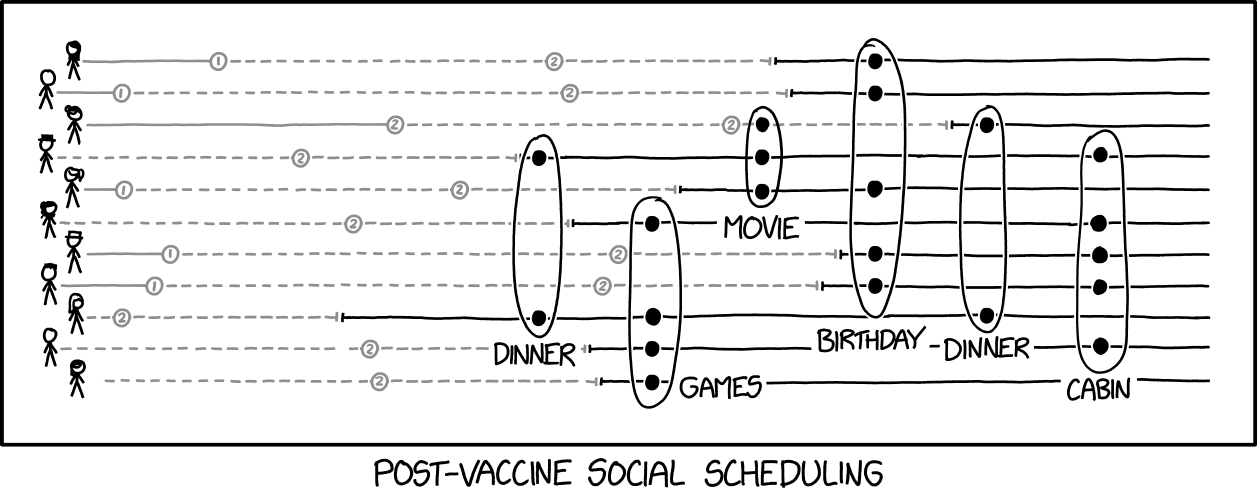
\includegraphics[width=5in]{post_vaccine_social_scheduling_2x.png}
\caption{``As if these problems weren't NP-hard enough.''}
\end{centering}
\end{figure}


\end{enumerate}
\end{document}
















